\documentclass[border=10pt]{standalone}
\usepackage{pgfplots}
\pgfplotsset{compat=newest}
\usepgfplotslibrary{fillbetween}
\begin{document}
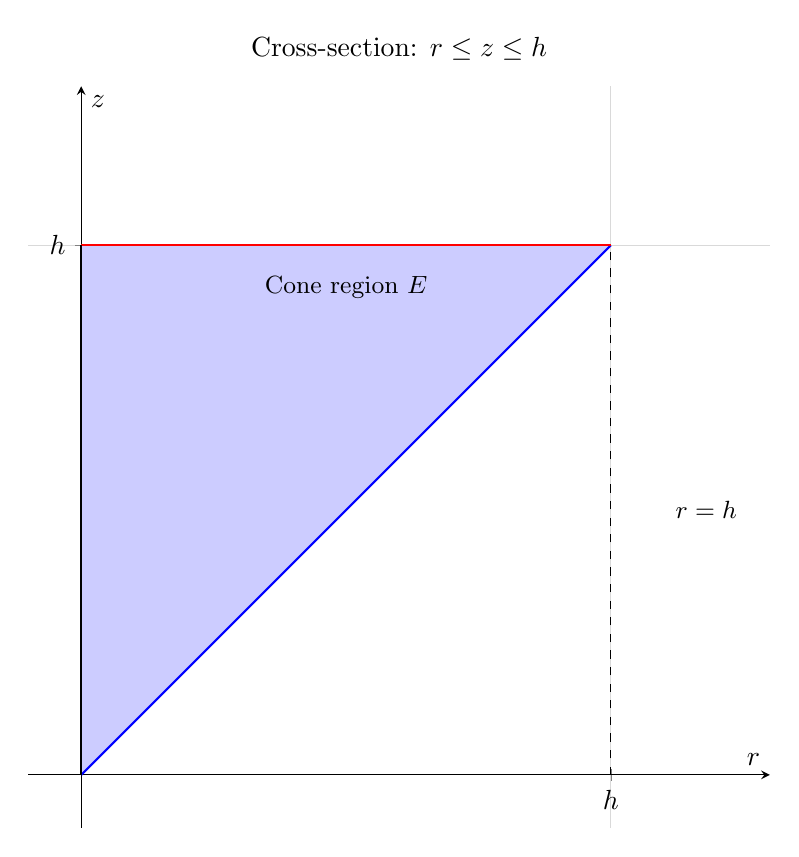
\begin{tikzpicture}
\begin{axis}[
    axis lines=middle,
    xlabel={$r$}, ylabel={$z$},
    xmin=-0.1, xmax=1.3, ymin=-0.1, ymax=1.3,
    xtick={1}, ytick={1},
    xticklabels={$h$}, yticklabels={$h$},
    width=11cm, height=11cm,
    title={Cross-section: $r \leq z \leq h$},
    grid=major, grid style={gray!30},
    legend pos=south east,
    samples=50, domain=0:1
]
\addplot[name path=lower, draw=blue, thick] {x};
\addplot[name path=upper, draw=red,  thick, forget plot] {1};
\addplot[blue!20] fill between[of=lower and upper];

\addplot[dashed, black] coordinates {(1,0) (1,1)};
\addplot[black, thick] coordinates {(0,0) (0,1)};

\node at (axis cs:0.5,0.92) {\small Cone region $E$};
\node at (axis cs:1.18,0.5) {\small $r=h$};
\end{axis}
\end{tikzpicture}
\end{document}
